\documentclass{article}

\usepackage[spanish]{babel}
\usepackage[utf8]{inputenc}
\usepackage{fancyhdr}
\usepackage{extramarks}
\usepackage{amsmath}
\usepackage{amsthm}
\usepackage{amsfonts}
\usepackage{tikz}
\usepackage[plain]{algorithm}
\usepackage{algpseudocode}
\usepackage{hyperref}
\usepackage{graphicx}
\usepackage{float}

\usetikzlibrary{automata,positioning}

%
% Basic Document Settings
%

\topmargin=-0.45in
\evensidemargin=0in
\oddsidemargin=0in
\textwidth=6.5in
\textheight=9.0in
\headsep=0.25in

\linespread{1.1}

\pagestyle{fancy}
\lhead{\hmwkAuthorName}

\setlength{\headheight}{35pt}

\chead{
	\parbox{0.8\textwidth}{
		\centering
		\hmwkClass\ (\hmwkClassInstructor)\\
		\hmwkTitle
}}

\rhead{\firstxmark}
\lfoot{\lastxmark}
\cfoot{\thepage}

\renewcommand\headrulewidth{0.4pt}
\renewcommand\footrulewidth{0.4pt}

\setlength\parindent{0pt}

%
% Create Problem Sections
%

\newcommand{\enterProblemHeader}[2]{
	\nobreak\extramarks{}{Problema \arabic{#1} continúa en la sig pág\ldots}\nobreak{}
	\nobreak\extramarks{Problema \arabic{#1} (continúa)}{Problema \arabic{#1} continúa en la sig pág\ldots}\nobreak{}
}

\newcommand{\exitProblemHeader}[2]{
	\nobreak\extramarks{Problema \arabic{#1}}{Problema \arabic{#1} continúa en la sig pág\ldots}\nobreak{}
	\stepcounter{#1}
	\nobreak\extramarks{Problema \arabic{#1}}{}\nobreak{}
}

\setcounter{secnumdepth}{0}
\newcounter{partCounter}
\newcounter{homeworkProblemCounter}
\setcounter{homeworkProblemCounter}{2}
\nobreak\extramarks{Problema \arabic{homeworkProblemCounter}}{}\nobreak{}

%
% Homework Problem Environment
%
% This environment takes an optional argument. When given, it will adjust the
% problem counter. This is useful for when the problems given for your
% assignment aren't sequential. See the last 3 problems of this template for an
% example.
%
\newenvironment{homeworkProblem}[2][-1]{
	\ifnum#1>0
	\setcounter{homeworkProblemCounter}{#1}
	\fi
	\def\currentProblemTitle{#2}
	\section{Problema \arabic{homeworkProblemCounter}: #2}
	\setcounter{partCounter}{1}
	\enterProblemHeader{homeworkProblemCounter}{#2}
}{
	\exitProblemHeader{homeworkProblemCounter}{\currentProblemTitle}
}
%
% Homework Details
%   - Title
%   - Due date
%   - Class
%   - Section/Time
%   - Instructor
%   - Author
%

\newcommand{\hmwkTitle}{Simulador del Tangent Bug\ \#2}
\newcommand{\hmwkDueDate}{21 de mayo de 2026}
\newcommand{\hmwkClass}{Planificación de movimientos de robots}
\newcommand{\hmwkClassInstructor}{Rafael Murrieta Cid}
\newcommand{\hmwkAuthorName}{\textbf{Andrés Alemán}}

%
% Title Page
%

\title{
	\vspace{2in}
	\textmd{\textbf{\hmwkClass:\ \hmwkTitle}}\\
	\normalsize\vspace{0.1in}\small{Due\ on\ \hmwkDueDate}\\
	\vspace{0.1in}\large{\textit{\hmwkClassInstructor}}
	\vspace{3in}
}

\author{\hmwkAuthorName}
\date{}

\renewcommand{\part}[1]{\textbf{\large Parte \Alph{partCounter}}\stepcounter{partCounter}\\}

%
% Various Helper Commands
%

% Useful for algorithms
\newcommand{\alg}[1]{\textsc{\bfseries \footnotesize #1}}

% For derivatives
\newcommand{\deriv}[1]{\frac{\mathrm{d}}{\mathrm{d}x} (#1)}

% For partial derivatives
\newcommand{\pderiv}[2]{\frac{\partial}{\partial #1} (#2)}

% Integral dx
\newcommand{\dx}{\mathrm{d}x}

% Alias for the Solution section header
\newcommand{\solution}{\textbf{\large Solución}}

% Probability commands: Expectation, Variance, Covariance, Bias
\newcommand{\E}{\mathrm{E}}
\newcommand{\Var}{\mathrm{Var}}
\newcommand{\Cov}{\mathrm{Cov}}
\newcommand{\Bias}{\mathrm{Bias}}

\begin{document}
	
%	\maketitle
	
%	\pagebreak
	
	\begin{homeworkProblem}{Programar Tangent Bug en un simulador.}
	
	\textbf{Repositorio del Proyecto:} \href{https://github.com/andresalemn/robotics-sandbox/tree/master/tangent_bug}{github.com/andresalemn/robotics-sandbox/tangent\_bug}
	
	\section{Resumen del Método: Algoritmo Tangent Bug}
	
	El algoritmo \textbf{Tangent Bug} es una técnica de planificación de trayectorias reactiva que permite a un robot navegar desde una posición inicial hasta una meta en un entorno con obstáculos desconocidos. A diferencia de algoritmos como Bug 1 o Bug 2, que dependen únicamente de sensores de contacto, Tangent Bug utiliza un sensor de rango (como un LIDAR o sonar) para detectar obstáculos a distancia, lo que le permite tomar decisiones más eficientes.
	
	El robot opera bajo una máquina de estados finitos con dos modos principales:
	
	\begin{enumerate}
		\item \textbf{Movimiento hacia el objetivo (Motion-to-Goal):} El robot intenta avanzar directamente hacia la meta. Mientras se mueve, escanea su entorno buscando "puntos tangentes". Estos puntos son discontinuidades en las lecturas del sensor que representan los bordes u esquinas de los obstáculos visibles. El robot selecciona el punto tangente que minimiza la suma de la distancia desde el robot al punto y desde el punto a la meta ($d(x, T_i) + d(T_i, q_{goal})$).
		
		\item \textbf{Seguimiento de fronteras (Boundary Following):} Si un obstáculo bloquea el camino directo y el robot no puede mejorar su distancia a la meta moviéndose hacia un punto tangente, entra en este modo. El robot bordea el obstáculo manteniendo una distancia constante. Durante este proceso, registra la distancia mínima ($d_{min}$) a la que ha estado de la meta.
	\end{enumerate}
	
	\textbf{Condición de salida:} El robot abandona el modo de seguimiento de fronteras cuando detecta un punto en el obstáculo que está más cerca de la meta que cualquier punto visitado anteriormente durante ese seguimiento ($d(x, q_{goal}) < d_{min}$) y tiene una línea de visión despejada hacia la meta.
	
	\section{Descripción del Simulador}
	
	Se implementó un simulador interactivo utilizando \textbf{Python} y la biblioteca \textbf{Pygame}. El simulador permite al usuario:
	\begin{itemize}
		\item Dibujar obstáculos poligonales de forma arbitraria.
		\item Definir la posición inicial del robot y la ubicación de la meta.
		\item Visualizar en tiempo real el comportamiento del algoritmo, incluyendo los rayos del sensor y los cambios de estado.
		\item Generar reportes gráficos automáticos y grabaciones de video de la simulación.
	\end{itemize}
	
	\subsection{Modelo del Sensor}
	El robot cuenta con un sensor de rango de 360$^\circ$ con un alcance finito $R$. El sensor emite 72 rayos (uno cada 5$^\circ$). Si un rayo impacta un obstáculo, devuelve la distancia; de lo contrario, devuelve el rango máximo $R$. Los puntos tangentes se identifican buscando saltos bruscos en las distancias de rayos adyacentes.
	
	\section{Resultados y Gráficas}
	
	Tras la ejecución del simulador, se generan gráficas que permiten analizar el desempeño del robot:
	
	\begin{itemize}
		\item \textbf{Distancia a la meta vs. Tiempo:} Muestra cómo disminuye la distancia a medida que el robot progresa. Los segmentos verdes indican movimiento hacia la meta y los naranjas indican seguimiento de obstáculos.
		\item \textbf{Pasos por estado:} Un gráfico de barras que cuantifica la eficiencia del algoritmo en términos de cuántos pasos fueron necesarios en cada modo.
		\item \textbf{Mapa de navegación:} Una representación visual de la trayectoria final sobrepuesta en el mapa de obstáculos, permitiendo verificar que no hubo colisiones y que se respetó la lógica del algoritmo.
	\end{itemize}
	
	\begin{table}[H]
		\centering
		\begin{tabular}{cc}
			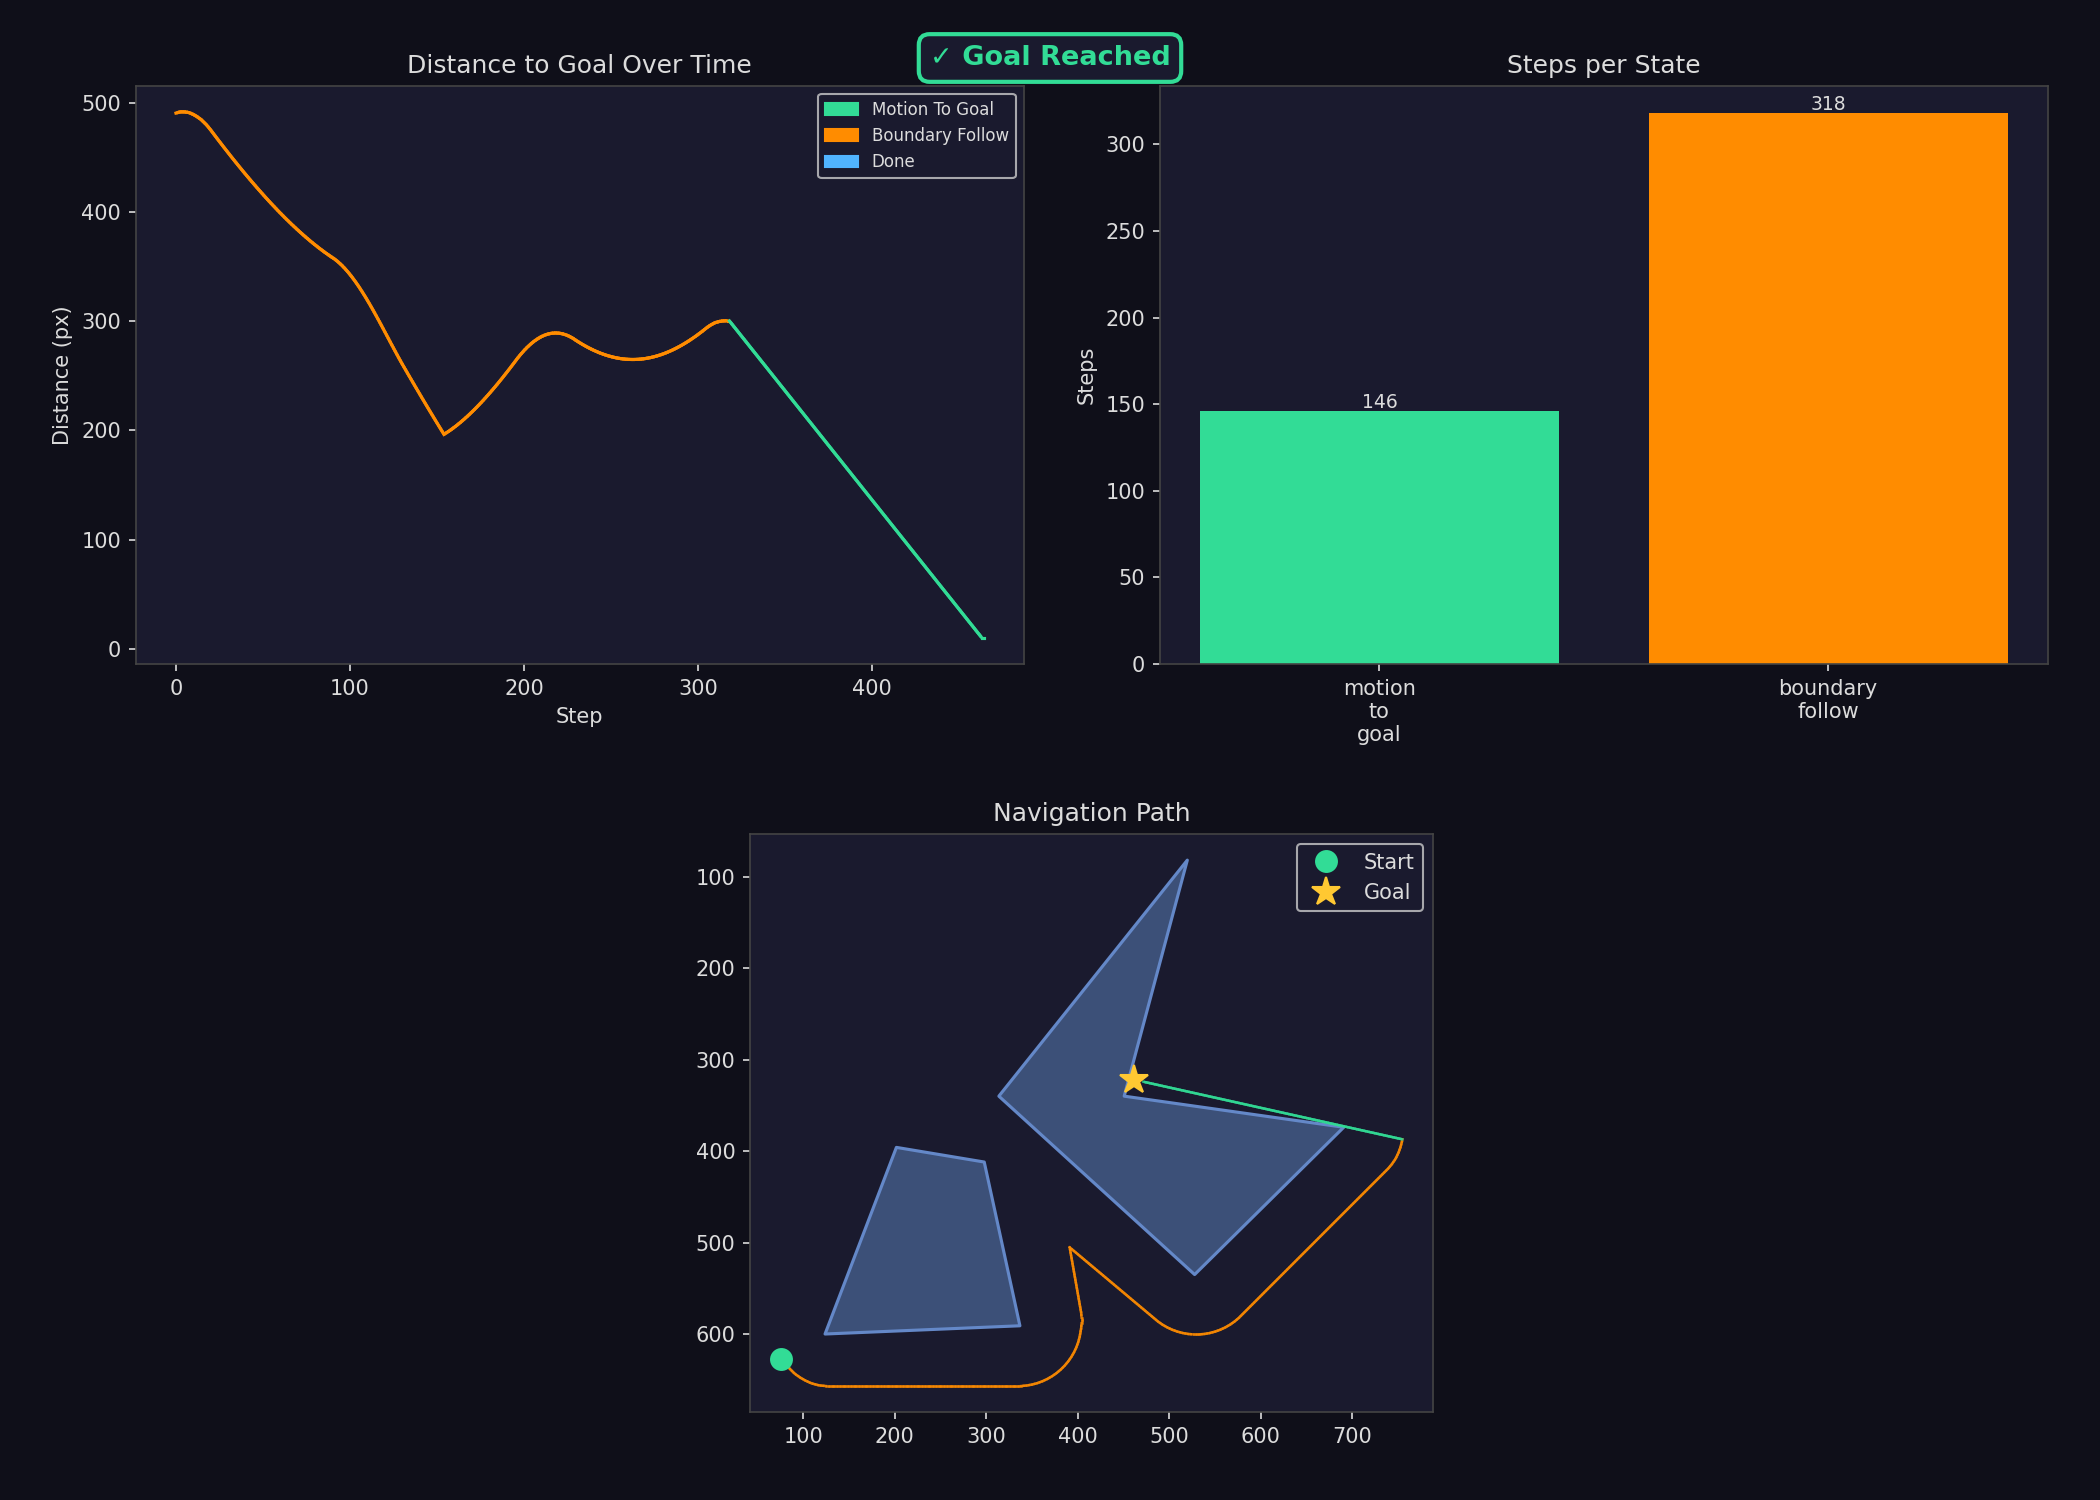
\includegraphics[width=0.45\textwidth]{report.png} & 
			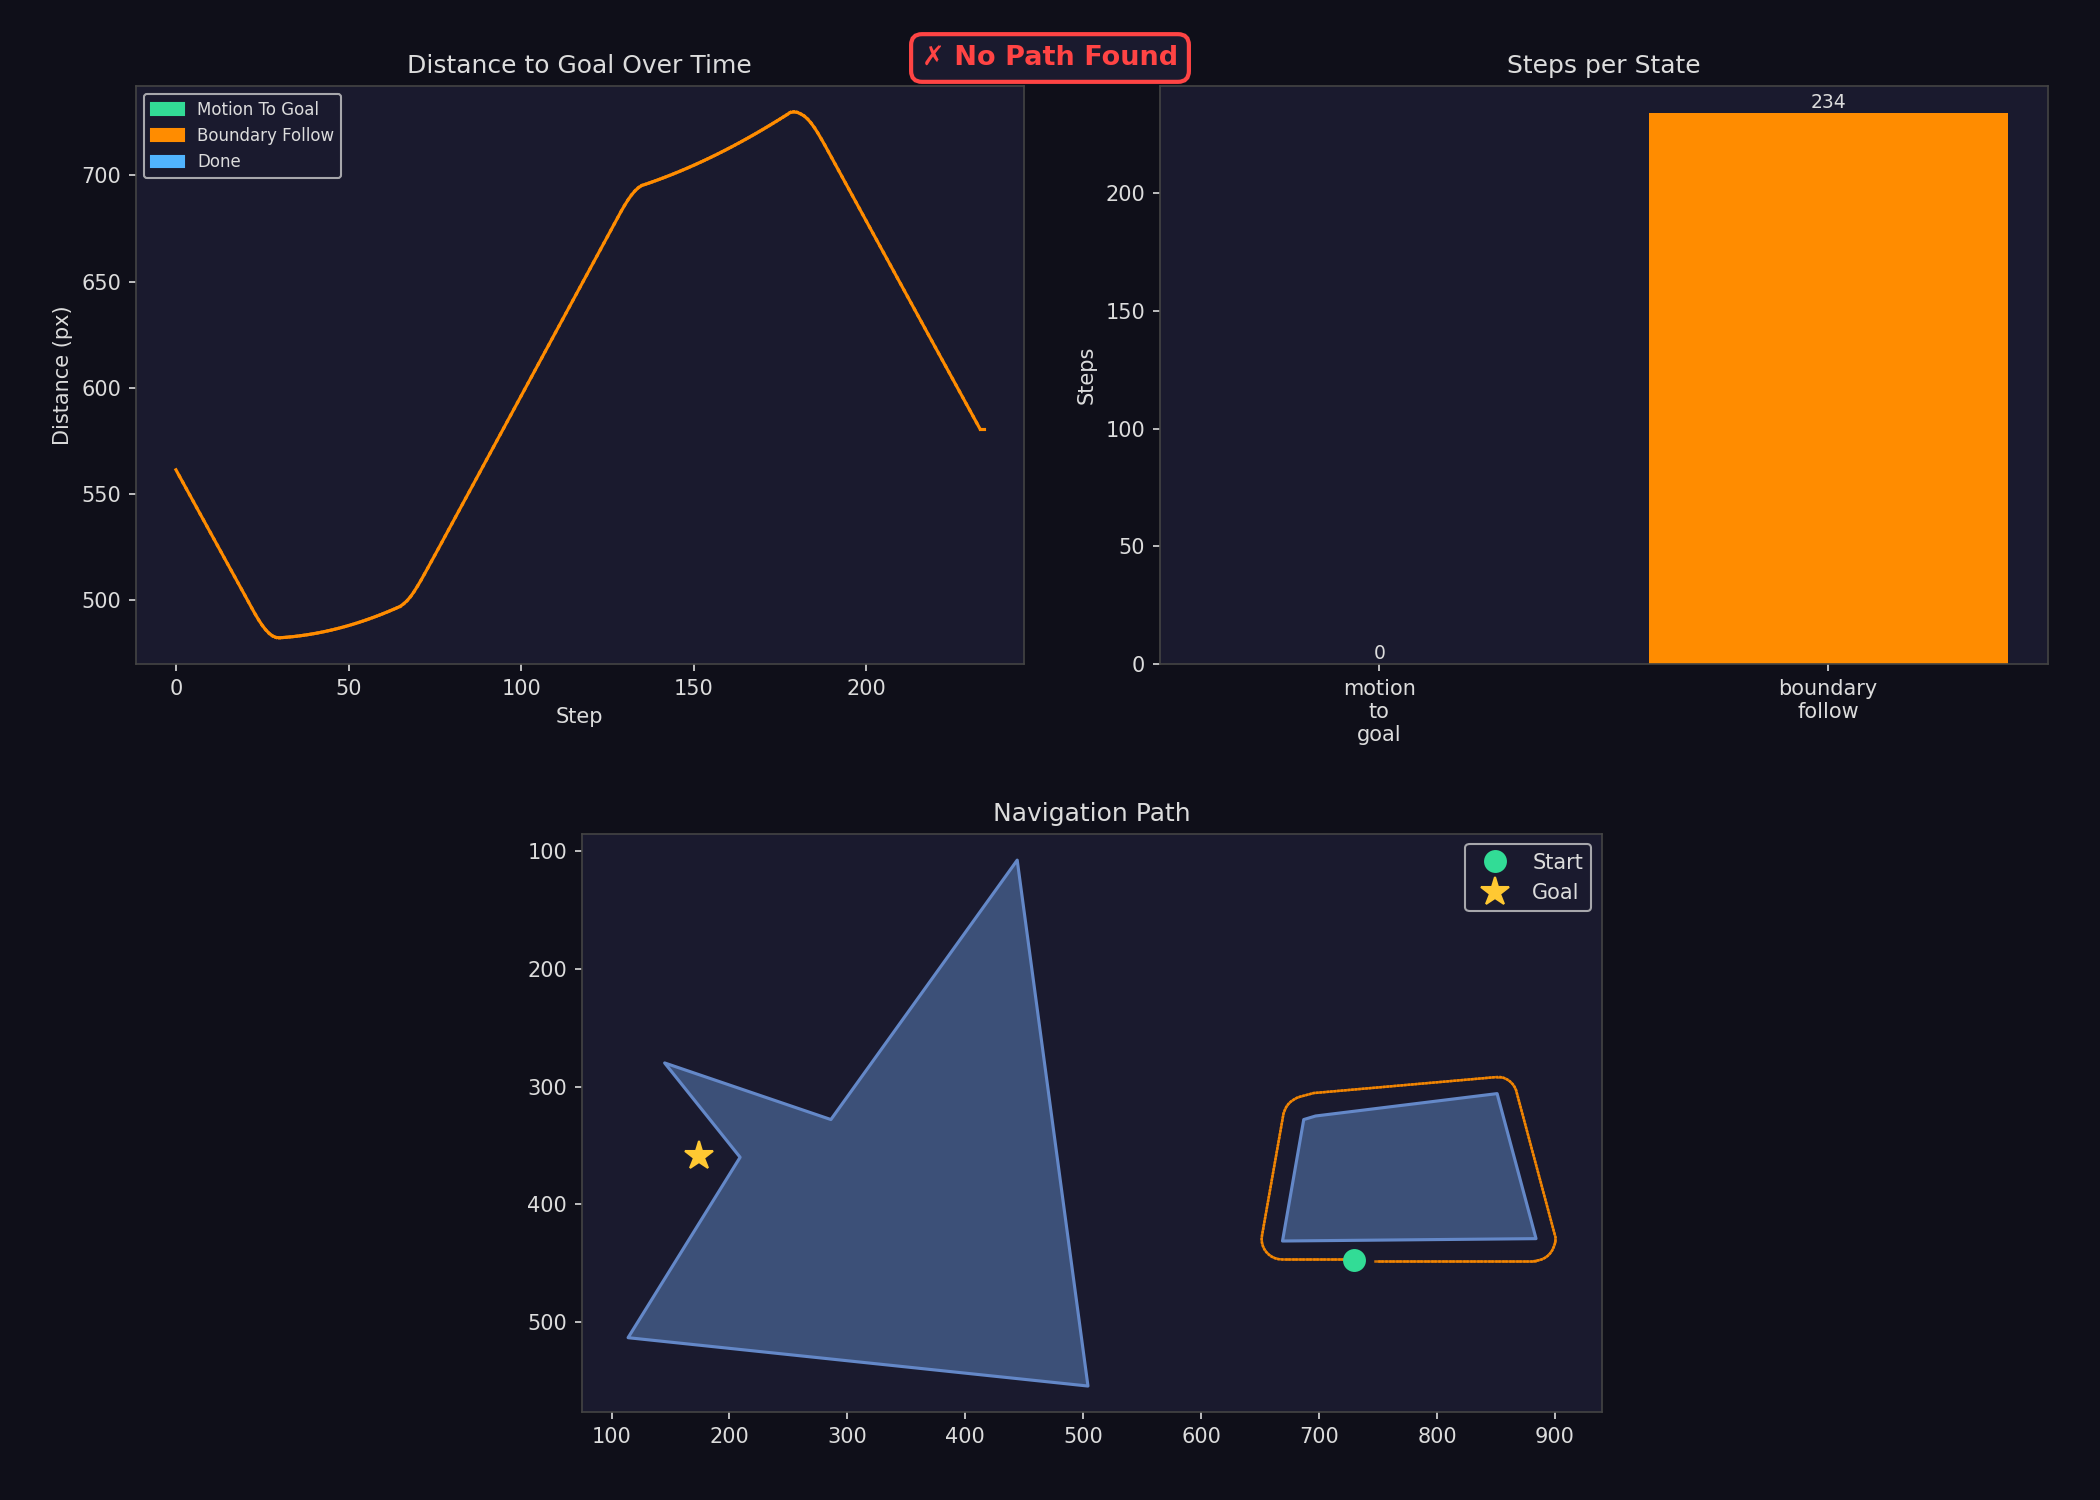
\includegraphics[width=0.45\textwidth]{report2.png} \\
			(a) Camino Encontrado & (b) No Path Found (Bucle detectado)
		\end{tabular}
		\caption{Reportes generados por el simulador para dos escenarios distintos.}
	\end{table}
	
	\section{Conclusiones}
	El algoritmo Tangent Bug demuestra ser significativamente más eficiente que los algoritmos Bug clásicos al aprovechar la información de rango. La capacidad de anticipar bordes de obstáculos permite realizar trayectorias más fluidas y reducir el tiempo dedicado al seguimiento de fronteras.
		
	\end{homeworkProblem}
	
	
\end{document}
